% title: Scheduling groups independent equations into parallel stages
% description: The original IR lists independent operations A and B before Join, which depends on both. Scheduling groups A and B into a parallel stage followed by Join. The dependencies remain unchanged.
\documentclass[tikz,border=5pt]{standalone}
\usetikzlibrary{arrows.meta}
\begin{document}
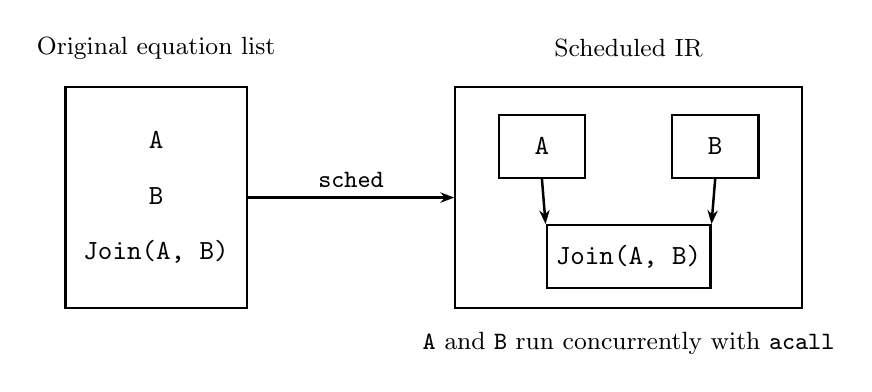
\begin{tikzpicture}[
    box/.style={draw, line width=0.8pt, minimum height=0.8cm,
                minimum width=2cm, align=center},
    flow/.style={-{Stealth[length=5pt]}, line width=0.9pt},
    note/.style={font=\small, align=center},
]

    \node[box, minimum width=2.3cm, minimum height=2.8cm] (original) at (0, 0)
        {\texttt{A}\\[8pt]\texttt{B}\\[8pt]\texttt{Join(A, B)}};
    \node[note] at (0, 1.9) {Original equation list};
    \node[box, minimum width=4.4cm, minimum height=2.8cm] (new) at (6, 0) {};
    \node[note] at (6, 1.9) {Scheduled IR};
    \node[box, minimum width=1.1cm] (a) at (4.9, 0.65) {\texttt{A}};
    \node[box, minimum width=1.1cm] (b) at (7.1, 0.65) {\texttt{B}};
    \node[box, minimum width=2cm] (join) at (6, -0.75) {\texttt{Join(A, B)}};
    \draw[flow] (a.south) -- (join.north west);
    \draw[flow] (b.south) -- (join.north east);
    \draw[flow] (original.east) -- node[above, note] {\texttt{sched}} (new.west);
    \node[note] at (6, -1.85) {\texttt{A} and \texttt{B} run concurrently with \texttt{acall}};
\end{tikzpicture}
\end{document}
